\documentclass[a4paper,12pt]{article}
\usepackage[polish]{babel}
\usepackage[T1]{fontenc}
\usepackage[utf8]{inputenc}
\usepackage{listings}
\usepackage{graphicx}
\usepackage{hyperref}
\usepackage{amsmath}
\usepackage{geometry}
\usepackage{enumitem}
\geometry{
    a4paper,
    left=25mm,
    right=25mm,
    top=20mm,
    bottom=25mm
}

\title{\textbf{Dokumentacja systemu \texttt{VecEdit}}}
\author{Zespół projektowy: \\
\small Adam Rogowski, Szymon Sawoń, Bartosz Siemaszkiewicz}
\date{\today}

\begin{document}

\maketitle
\tableofcontents

\section{Wstęp}

\texttt{VecEdit} to aplikacja (napisana w~\textbf{C++20}) służąca do edycji prostych
grafik wektorowych. Umożliwia rysowanie, modyfikowanie, grupowanie oraz klonowanie
obiektów graficznych (takich jak prostokąty, okręgi czy wielokąty). 
Program korzysta z biblioteki \textbf{raylib} (w wersji 5.5) do wyświetlania okna, 
rysowania figur na ekranie oraz pobierania zdarzeń wejściowych od użytkownika 
(klawiatura, mysz). Do tworzenia interfejsu graficznego w trybie \emph{immediate mode}
używana jest biblioteka \textbf{RayGui}.  

Aplikacja pozwala na:
\begin{itemize}
    \item rysowanie i edycję kształtów (w tym zmianę koloru, obrysu, przezroczystości),
    \item przesuwanie i skalowanie figur,
    \item grupowanie obiektów (\texttt{FigureGroup}),
    \item cofanie (\texttt{undo}) i ponawianie (\texttt{redo}) operacji dzięki wzorcowi \emph{Command},
    \item zapisywanie projektów do plików wektorowych (\texttt{SVG}) i \emph{bitmapowych} (\texttt{PNG}),
    \item otwieranie, zamykanie i przełączanie się między wieloma zakładkami dokumentów.
\end{itemize}

\section{Wzorce projektowe i ich zastosowanie}

Poniżej przedstawiono zastosowane wewnątrz aplikacji wzorce projektowe,
z uwzględnieniem istotnych elementów w~kodzie oraz komentarzy dotyczących
możliwych zmian (tzw. \emph{wektora zmian}).

\subsection{Kompozyt (\emph{Composite})}
\begin{itemize}
    \item \textbf{Cel:} Umożliwienie traktowania pojedynczych obiektów
    (figury) i grup obiektów (grupy figur) w sposób jednolity, dzięki interfejsowi
    \texttt{Figure}. 
    \item \textbf{Struktura:} 
    \begin{itemize}
      \item \texttt{figure} -- przestrzeń nazw, w której znajdują się klasy komponentów
      \item \texttt{Figure} -- interfejs \emph{komponentu}. Posiada m.in. metody typu 
      \texttt{accept(visitor)}, które w~implementacjach \emph{Composite} przekazują
        wywołanie wszystkim dzieciom. (\verb|src/figure/Figure.h|)
      \item \texttt{FigureGroup} -- \emph{kompozyt}, zawiera wektor \texttt{children}
      oraz metody \texttt{addChild(...)} itp. (\verb|src/figure/FigureGroup.h|)
      \item \texttt{RectFigure}, \texttt{CircleFigure}, \texttt{PolyFigure} -- 
      \emph{konkretne komponenty (liście)}, nie posiadają dzieci. (\verb|src/figure/*Figure.h|)
    \end{itemize}
    \item \textbf{Użycie:} 
    \begin{itemize}
      \item W edytorze (\texttt{Editor} - \verb|src/ui/Editor.cpp|) przy \texttt{groupFigures()} i \texttt{ungroupFigures()}
      łączymy/rozbijamy figury w drzewiastą strukturę.
      \item \texttt{accept(visitor)} w \texttt{FigureGroup} wywołuje
        \texttt{accept} u wszystkich dzieci, co integruje się z~\emph{Visitor}. (np. \verb|ui::Editor::renderMainContent()|)
    \end{itemize}
    \item \textbf{Wektor zmian:} Dodanie kolejnych typów figur nie wymaga zmian
      w \texttt{FigureGroup}, wystarczy zaimplementować metody interfejsu 
      \texttt{Figure} - najlepiej dziedzicząc po \texttt{FigureGroup}.
\end{itemize}

\subsection{Metoda wytwórcza (\emph{Factory Method})}
\begin{itemize}
    \item \textbf{Cel:} Abstrakcja sposobu tworzenia obiektów. 
    W naszym projekcie służy do tworzenia odpowiedniej implementacji 
    \texttt{PointEditor} w metodzie \texttt{Figure::makePointEditor()}.
    \item \textbf{Struktura i użycie:}
    \begin{itemize}
        \item \texttt{Figure} deklaruje wirtualną metodę \texttt{makePointEditor()}, 
        która w podklasach (\texttt{RectFigure}, \texttt{CircleFigure}, \dots) zwraca
        odpowiedni edytor (np. \texttt{RectFigurePointEditor}).
        \item \texttt{Editor} korzysta z tej metody, by pobierać adapter 
        do edycji punktów figury, nie wiedząc \emph{jaki to} konkretnie edytor.
    \end{itemize}
    \item \textbf{Wektor zmian:} Nowy typ figury (np. \texttt{StarFigure}) 
    wystarczy wyposażyć w swoją implementację \texttt{makePointEditor()}, 
    zwracając własną implementację \texttt{PointEditor} np. \texttt{StarFigurePointEditor}.
\end{itemize}

\subsection{Strategia (\emph{Strategy})}
\begin{itemize}
    \item \textbf{Cel:} Definiowanie wymiennych algorytmów/akcji, 
    które można przypisać do przycisków lub skrótów klawiaturowych (np. \emph{undo}, \emph{redo}).
    \item \textbf{Kluczowe elementy:}
    \begin{itemize}
        \item \texttt{ui::strategy} -- przestrzeń nazw, w której znajdują się klasy strategii
        \item \texttt{Strategy<...>} -- generyczny interfejs (plik \texttt{Strategy.h}) 
          -- argumenty szablonu odnoszą się do typów argumentów przekazywanych 
          podczas wywołania strategi, 
        \item \texttt{UndoStrategy}, \texttt{RedoStrategy}, \texttt{SetSelectStrategy} 
        itp. -- konkretne strategie używane przez guziki i skróty klawiszowe,
        \item \texttt{FunctorStrategy<...>} -- pozwala zdefiniować strategię
        w oparciu o lambda/domknięcie (\emph{closure}), bez tworzenia nowej podklasy.
    \end{itemize}
    \item \textbf{Użycie:} 
    \begin{itemize}
      \item W \texttt{AppUi} (np. \verb|ui::AppUi::setupUndoRedoButtons()|)
        do \texttt{IconButton} lub \texttt{KeyboardShortcut} przypisujemy 
       strategię. Np. \texttt{auto str = std::make\_shared<UndoStrategy>(editor)},
       a w innym miejscu \texttt{addShortcut(str, KEY\_Z, mod)}.
       \item W \texttt{FunctorStrategy} wystarczy przekazać lambdę, 
       np. \texttt{FunctorStrategy<>\{[this]() \{ editor->exportDocument("png"); \}\}}.
    \end{itemize}
    \item \textbf{Wektor zmian:} Aby dodać nową prostą akcję, można utworzyć
    instancję \texttt{FunctorStrategy} z odpowiednim wyrażeniem lambda; 
    dla bardziej złożonych przypadków — osobną klasę dziedziczącą po \texttt{Strategy}.
\end{itemize}

\subsection{Adapter}
\begin{itemize}
    \item \textbf{Cel:} Udostępnienie wspólnego interfejsu edycji punktów figur 
    (\texttt{PointEditor}) mimo iż każda figura ma odmienne właściwości i sposób 
    ich zmiany.
    \item \textbf{Struktura i użycie:}
    \begin{itemize}
      \item \texttt{figure::adapter} -- przestrzeń nazw, w której znajdują się klasy adapterów
      \item \texttt{PointEditor} -- interfejs z metodami \texttt{getEditPoints()}
      i \texttt{updatePointPosition(...)},
      \item \texttt{RectFigurePointEditor}, \texttt{CircleFigurePointEditor}, 
      \texttt{PolyFigurePointEditor} -- adaptery do konkretnych figur,
      \item Każdy adapter \emph{zwraca} (np. w \texttt{getEditPoints()}) położenia uchwytów 
      charakterystyczne dla swojej figury (np. promień dla koła).
    \end{itemize}
    \item \textbf{Wektor zmian:} Dodanie nowego kształtu wymaga stworzenia
    nowego adaptera do edycji, a sama logika \texttt{Editor} (obsługująca \texttt{PointEditor})
    nie musi być zmieniana.
\end{itemize}

\subsection{Odwiedzający (\emph{Visitor})}
\begin{itemize}
    \item \textbf{Cel:} Oddzielenie logiki przetwarzania figur (np. rysowania, 
    zapisu do pliku) od samych klas figur.
    \item \textbf{Struktura i użycie:}
    \begin{itemize}
      \item \texttt{figure::visitor} -- przestrzeń nazw, w której znajdują się klasy odwiedzających
      \item \texttt{FigureVisitor} -- interfejs odwiedzającego (\verb|src/figure/visitor/FigureVisitor.h|), 
      \item \texttt{RendererVisitor} (renderuje figury na ekranie) (\verb|src/figure/visitor/RendererVisitor.cpp|),
      \item \texttt{SvgSerializerVisitor} (zapisuje wektorowo do pliku SVG),
      \item \texttt{BitmapRendererVisitor} (obsługa zapisu do formatów bitmapowych np. \texttt{PNG}).
      \item Metoda \texttt{accept(visitor)} w \texttt{Figure} (bądź \texttt{FigureGroup})
      wywołuje \texttt{visitor.visit(...)} odpowiedniego typu.
    \end{itemize}
    \item \textbf{Wektor zmian:} Dodanie kolejnej operacji (np. liczenie pola figur)
    wymaga utworzenia nowej klasy odwiedzającego, bez modyfikacji istniejących figur. Z kolei
    dodanie nowej figury pociąga za sobą modyfikację wszystkich odwiedzających tak
    by obsłużyć odwiedzenie nowego rodzaju figury.
\end{itemize}

\subsection{Prototyp (\emph{Prototype})}
\begin{itemize}
    \item \textbf{Cel:} Możliwość tworzenia nowych instancji obiektów (figur)
      poprzez klonowanie bez tworzenia zależności pomiędzy kodem wywołującym 
      a konkretną klasą, której obiekt jest tworzony.
    \item \textbf{Struktura i użycie:}
    \begin{itemize}
      \item \texttt{FigureBase<FigureType>} posiada wirtualną metodę \texttt{clone()},
      a w podklasach (\texttt{RectFigure}, \texttt{CircleFigure} itp.) implementuje 
      tworzenie kopii obiektu \emph{danego} typu.
      \item W \texttt{Editor::processModeInsert()} tworzymy nową figurę poprzez
      sklonowanie istniejącego prototypu (figura-prototyp jest wcześniej
      ustawiona przez\break \texttt{SetFigureInsertStrategy}).
    \end{itemize}
    \item \textbf{Wektor zmian:} Każda klasa dziedzicząca z \texttt{FigureBase<FigureType>}
      automatycznie dziedziczy implementację operacji klonowania (\verb|src/figure/FigureBase.h|: \verb|figure::FigureBase<FigureType>::clone()|) pozwalającej na tworzenie
    nowych instancji typu \texttt{FigureType}.
\end{itemize}

\section{Opis użytych bibliotek i narzędzi}

\subsection{Raylib (5.5)}
W projekcie korzystamy z \textbf{Raylib} (\verb|https://www.raylib.com/|) w wersji 5.5, która zapewnia:
\begin{itemize}
    \item Wyświetlanie okna aplikacji w trybie 2D (np. \texttt{InitWindow}, \texttt{WindowShouldClose}),
    \item Funkcje do rysowania podstawowych kształtów (np. \texttt{DrawRectangle}, \texttt{DrawCircle}),
    \item Obsługę zdarzeń wejściowych (np. kliknięcia myszą (\texttt{IsMouseButtonPressed}), klawisze (\texttt{IsKeyDown})),
    \item Zapisywanie wyrenderowanej bitmapy do pliku (np. \texttt{ExportImage}).
\end{itemize}

\subsection{RayGui} 

Używamy \textbf{RayGui} (\verb|https://github.com/raysan5/raygui|) -- dodatek do Raylib, która wspiera tworzenie interfejsu
graficznego w tzw. \emph{immediate mode} — przyciski, suwaki i teksty
generowane są bezpośrednio podczas rysowania każdej klatki i natychmiastowo
obsługiwana jest ich interakcja. Umożliwia to proste tworzenie intefejsów
(dodanie jednej kontrolki to wywołanie jednej funkcji np. \texttt{GuiButton})
użytkownika jednocześnie pozwalając nam stworzyć własny szkielet wzorców
projektowych obługujących ten interfejs.

\subsection{C++20 i CMake}
\begin{itemize}
    \item \textbf{C++20} — W projekcie używamy \texttt{std::filesystem} do
      obsługi plików, \texttt{std::format} do wygodnego formatowania tekstu,
      \texttt{std::ranges} to operacji na kolekcjach. Wspierane są kompilatory
      GCC (14.2.1) i clang (18.1.8).

    \item \textbf{CMake 3.29} — Plik \texttt{CMakeLists.txt} konfiguruje system
      budowania i podczas generowania konfiguracji projektu (np. dla
      \texttt{GNU Make} lub \texttt{Ninja}) automatycznie pobiera
      \texttt{Raylib} z GitHuba.
\end{itemize}

\section{Instrukcja użytkownika}

\subsection{Uruchomienie programu}
\texttt{VecEdit} można uruchomić:
\begin{itemize}
    \item \textbf{Z gotowego pliku wykonywalnego}: na platformie Windows lub Linux
    dostarczamy \emph{executable} w folderze \texttt{bin/}.
    \item \textbf{Z linii poleceń po kompilacji}: np.
\begin{verbatim}
cd build
./VecEdit
\end{verbatim}
\end{itemize}

\subsection{Interfejs programu — krótki opis}

\begin{figure}[h!]
    \centering
    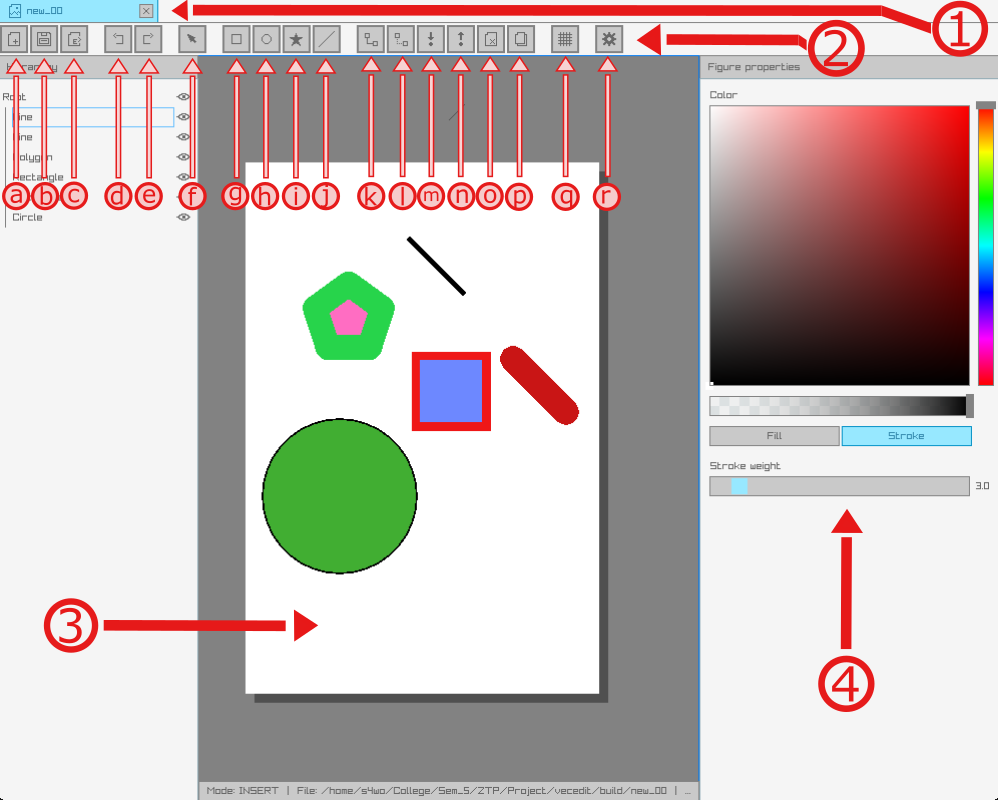
\includegraphics[width=0.75\textwidth]{./vecedit_screenshot.png}
    \caption{Przykładowy widok programu.}
    \label{fig:screenshot}
\end{figure}

\noindent Oznaczenia na zrzucie:
\begin{enumerate}
    \item \textbf{Pasek zakładek dokumentów} — wybór otwartego projektu, 
    możliwość zamknięcia karty.
    \item \textbf{Pasek narzędzi} (z przyciskami \textbf{od A do S}):
    \begin{enumerate}[label=\alph*)]
        \item \textbf{New} (skrót \texttt{Ctrl+N}) — tworzy nowy dokument.
        \item \textbf{Save} (skrót \texttt{Ctrl+S}) — zapisuje obecny dokument do \texttt{SVG}.
        \item \textbf{Export} (skrót \texttt{Ctrl+E}) — eksport do \texttt{PNG}.
        \item \textbf{Undo} (skrót \texttt{Ctrl+Z}) - cofnięcie zmian
        \item \textbf{Redo} (skrót \texttt{Ctrl+Y}) - przywrócenie zmian
        \item \textbf{Select} (skrót \texttt{Q}) — narzędzie zaznaczania figur.
        \item \textbf{Insert Rectangle} (skrót \texttt{R}) — wstawianie prostokąta.
        \item \textbf{Insert Circle} (skrót \texttt{E}) — wstawianie koła.
        \item \textbf{Insert Polygon} (skrót \texttt{T}) — wstawianie wielokąta gwiazdy.
        \item \textbf{Insert Line} (skrót \texttt{L}) — wstawianie linii.
        \item \textbf{Group} (skrót \texttt{Ctrl+G}) - grupowanie zaznaczonych figury obiektów.
        \item \textbf{Ungroup} (skrót \texttt{Ctrl+U}) - odgrupowanie obiektów.
        \item \textbf{Move Lower} (skrót \texttt{PageDown}) - przeniesienie zaznaczonej figury w dół w hierarchii obiektów.
        \item \textbf{Move Higher} (skrót \texttt{PageUp}) - przeniesienie zaznaczonej figury w górę w hierarchii obiektów.
        \item \textbf{Delete Figure} (skrót \texttt{Delete}) - usunięcie zaznaczonej figury.
        \item \textbf{Duplicate Figure} (\texttt{Ctrl+D}) - zduplikowanie figury.
        \item \textbf{Toggle Grid} (\texttt{Ctrl+I}) — włączenie/wyłączenie przyciągania do siatki.
        \item \textbf{Document Properties} (\texttt{Ctrl+.}) — otwiera panel właściwości dokumentu (nazwa pliku i rozmiar płótna).
    \end{enumerate}
    \item \textbf{Obszar roboczy} — kliknięcie w tym obszarze lewym przyciskiem
      myszy wstawia figurę (jeśli wybrano narzędzie \emph{Insert}) lub zaznacza
      figurę (jeśli wybrano narzędzie \emph{Select} - trzymając Shift można
      zaznaczać wiele figur). Koło myszy pozwala na przybliżanie i oddalanie
      widoku jak również podczas trzymania Shift na przesuwanie widoku.
    \item \textbf{Panel właściwości} (z boku lub w oknie) — służy do zmiany 
    kolorów, grubości obrysu i przezroczystości dla wybranej figury.
\end{enumerate}

\section{Instrukcja instalacji i kompilacji}

Kompilacja ze źródłeł odbywa się w następujących krokach:

\begin{enumerate}
    \item \textbf{Rozpakowanie zip} - źródła projektu dostarczone są w archiwów zip, które należy rozpakować. \textbf{TODO: dodać dokładną nazwę folderu ze źródłami}
    \item \textbf{Kompilacja z użyciem CMake}
    \begin{itemize}
      \item  \textbf{W linii poleceń} - z wykorzystaniem \texttt{GNU Make} (proces opisany również w \texttt{README.md})
    \begin{verbatim}
    mkdir build
    cd build
    cmake ..  # ten krok może długo potrwać, ponieważ pobiera Raylib
    make
    \end{verbatim}
    \item \textbf{Kompilacja z użyciem środowiska CLion}:
        \begin{enumerate}
            \item Po zaimportowaniu projektu wykonać File->Reload CMake Project
            \item Następnie po ładowaniu można skompilować i uruchomić projekt za pomocą 
                przycisku "Run" lub \texttt{SHIFT+F10}
            \item Dodatkowo w folderze \texttt{vecedit/cmake-build-debug} jest
                plik .exe.
        \end{enumerate}
    \end{itemize}
    \item \textbf{Uruchomienie}: Po kompilacji w folderze \texttt{build} znajduje się 
    plik \texttt{VecEdit} (Linux/macOS) lub \texttt{VecEdit.exe} (Windows). 
    Można go uruchomić z wiersza poleceń lub przez dwuklik. 
\end{enumerate}

\section{Podział pracy w zespole}

\paragraph{Adam Rogowski}
\begin{itemize}
    \item \textbf{Composite} (\texttt{FigureGroup}): stworzenie klasy grupującej figury i zarządzanie hierarchią dzieci (w tym obsługa zagnieżdżonych grup).
    \item \textbf{Command} (w tym \texttt{RemoveFiguresCommand}, \texttt{GroupFiguresCommand} i \texttt{CommandManager}): implementacja głównego mechanizmu \texttt{undo}/\texttt{redo}, obejmująca tworzenie i cofanie poleceń.
    \item \textbf{Zarządzanie warstwami i blokowaniem figur}: dodatkowo rozbudował \texttt{Editor} o możliwość przesuwania obiektów między warstwami oraz blokowania/odblokowywania figur w drzewie.
    \item \textbf{Interfejs użytkownika} (\texttt{AppUi}, \texttt{Toolbar}): stworzenie paska narzędzi (z przyciskami od \texttt{New} do \texttt{Settings}), logika rozmieszczania widgetów i współpracy z \texttt{Editor} (m.in. przełączanie trybów \emph{insert} / \emph{select}).
\end{itemize}

\paragraph{Szymon Sawoń}
\begin{itemize}
    \item \textbf{Strategy}: implementacja akcji takich jak \texttt{SetSelectStrategy}, \texttt{OpenDocumentStrategy} oraz \texttt{FunctorStrategy} (do prostych poleceń tworzonych w oparciu o wyrażenia lambda).
    \item \textbf{Prototype}: w \texttt{FigureBase<>} oraz poszczególnych figurach (\texttt{RectFigure}, \texttt{CircleFigure} itp.) wdrożył metodę \texttt{clone()} pozwalającą na klonowanie obiektów bez znajomości ich typu.
    \item \textbf{Obsługa skrótów klawiaturowych} (\texttt{KeyboardShortcut}): mapowanie klawiszy na odpowiednie strategie (np. \texttt{Ctrl+N} na \texttt{NewDocumentStrategy}), przechowywanie listy skrótów i wywoływanie ich w pętli głównej.
    \item \textbf{Interfejs użytkownika} (\texttt{AppUi}, \texttt{Toolbar}): stworzenie paska narzędzi (z przyciskami od \texttt{New} do \texttt{Settings}), logika rozmieszczania widgetów i współpracy z \texttt{Editor} (m.in. przełączanie trybów \emph{insert} / \emph{select}).
\end{itemize}

\paragraph{Bartosz Siemaszkiewicz}
\begin{itemize}
    \item \textbf{Visitor}: implementacja \texttt{RendererVisitor} (rysowanie figur), \texttt{SvgSerializerVisitor} (eksport do \texttt{SVG}) oraz \texttt{BitmapRendererVisitor} (eksport do \texttt{PNG}).
    \item \textbf{Prototype}: w \texttt{FigureBase<>} oraz poszczególnych figurach (\texttt{RectFigure}, \texttt{CircleFigure} itp.) wdrożył metodę \texttt{clone()} pozwalającą na klonowanie obiektów bez znajomości ich typu.
    \item \textbf{Obsługa zapisywania do plików} (\texttt{SVG} i \texttt{PNG}): integracja z \texttt{Editor} i \texttt{Document}, przygotowanie procesu serializacji (np. \texttt{SvgSerializerVisitor}) i eksportowania całości sceny w wybranym formacie.
    \item \textbf{Interfejs użytkownika} (\texttt{AppUi}, \texttt{Toolbar}): stworzenie paska narzędzi (z przyciskami od \texttt{New} do \texttt{Settings}), logika rozmieszczania widgetów i współpracy z \texttt{Editor} (m.in. przełączanie trybów \emph{insert} / \emph{select}).
\end{itemize}

\section{Podsumowanie}
\texttt{VecEdit} stanowi przykład aplikacji, w~której zastosowanie wielu wzorców
projektowych (kompozyt, metoda wytwórcza, strategia, adapter, odwiedzający,
prototyp i command) umożliwia elastyczną i czytelną strukturę kodu:
\begin{itemize}
    \item \textbf{Composite} — wspólna obsługa figur i grup (hierarchii),
    \item \textbf{Factory Method} — tworzenie edytorów punktów figur,
    \item \textbf{Strategy} — łatwe definiowanie akcji dla GUI (także w postaci \texttt{FunctorStrategy}),
    \item \textbf{Adapter} — jednolite API do edycji różnych typów figur,
    \item \textbf{Visitor} — rozdzielenie logiki rysowania, serializacji i bitmap,
    \item \textbf{Prototype} — proste klonowanie figur,
    \item \textbf{Command} — mechanizm cofania i ponawiania operacji.
\end{itemize}

Dzięki temu kod można łatwo rozwijać (dodawać nowe rodzaje figur, strategie, odwiedzających) 
i utrzymywać.

\vspace{1em}
\noindent
\textbf{Miłego korzystania z \texttt{VecEdit}!}

\end{document}

